\section{Additional figures}
\label{app:extra_figs}

This appendix collects the parameter extrapolations, the factorization test on the lattice data and the amplitude data at the two highest momenta.

\subsection{Extrapolation of the fit parameters}
\label{app:param_extrap}

Figs.~\ref{fig:param_extrap} and~\ref{fig:param_extrap_j} show the extrapolation of the twelve fit parameters to $\hat\zeta\to\infty$ (Sec.~\ref{sec:zeta_extrapolation}): $a$ and $c$ in the first, $j$ and $d$ in the second.

\begin{figure*}[!p]
\centering
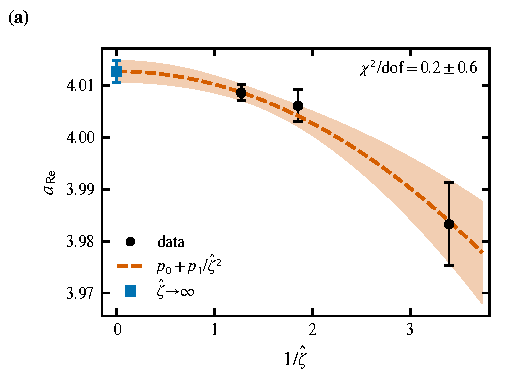
\includegraphics[width=\panelw]{figures/panels/extrap/par_ReA2B_a.pdf}\hfill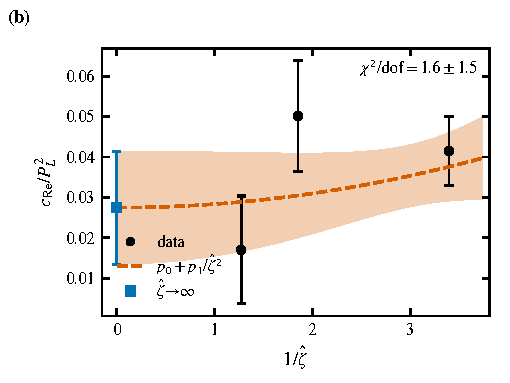
\includegraphics[width=\panelw]{figures/panels/extrap/par_ReA2B_c.pdf}\par
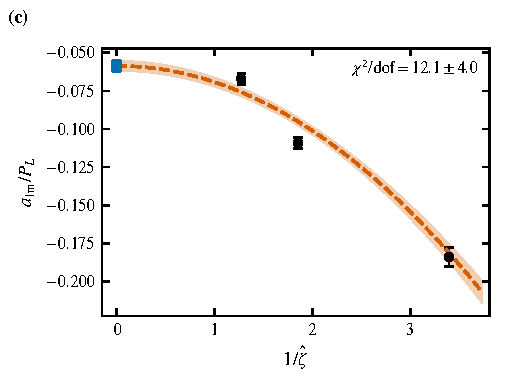
\includegraphics[width=\panelw]{figures/panels/extrap/par_ImA2B_a.pdf}\hfill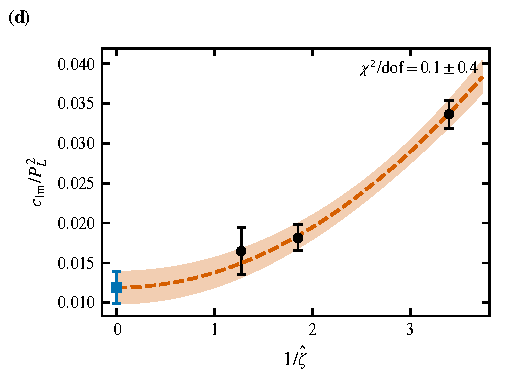
\includegraphics[width=\panelw]{figures/panels/extrap/par_ImA2B_c.pdf}\par
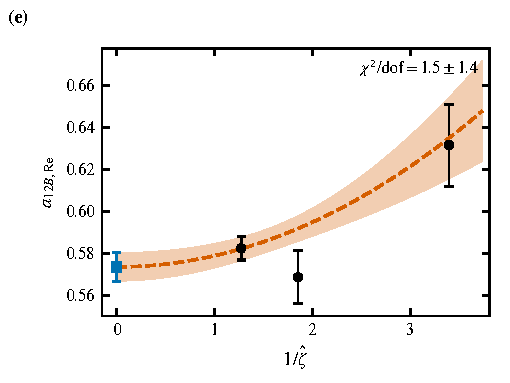
\includegraphics[width=\panelw]{figures/panels/extrap/par_ReA12B_a.pdf}\hfill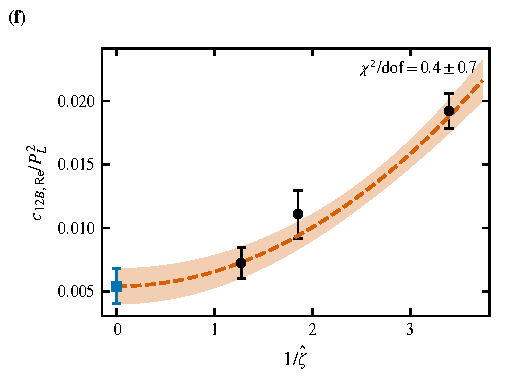
\includegraphics[width=\panelw]{figures/panels/extrap/par_ReA12B_c.pdf}
\caption{Extrapolation of the fit parameters $a$ and $c$ to $\hat\zeta\to\infty$ using $P_L=-2,-3,-4$ (black), with the ansatz $p_0+p_1/\hat\zeta^2$ (red dashed, band) and the extrapolated value (blue square). Panels (a, b) are for $\tAmp_{2B}^{\text{Re}}$, (c, d) for $\tAmp_{2B}^{\text{Im}}$ and (e, f) for $\tAmp_{12B}^{\text{Re}}$. Each panel gives the Jackknife $\chi^2/\text{dof}$. The parameters $c$ are shown rescaled by $1/P_L^2$ and the coefficient $a$ of $b_L$ in $\tAmp_{2B}^{\text{Im}}$ by $1/P_L$.}
\label{fig:param_extrap}
\end{figure*}

\begin{figure*}[!p]
\centering
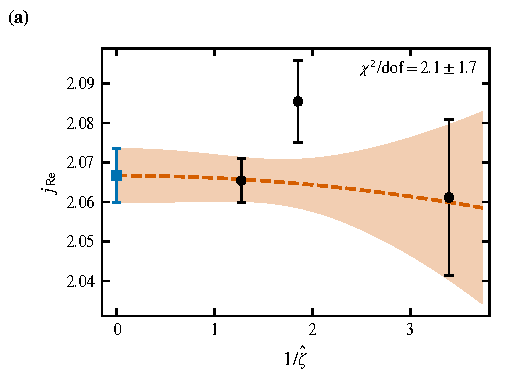
\includegraphics[width=\panelw]{figures/panels/extrap/par_ReA2B_j.pdf}\hfill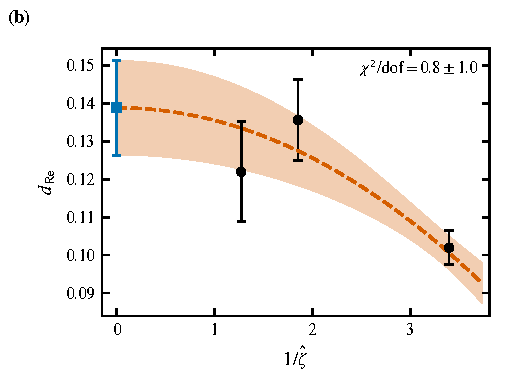
\includegraphics[width=\panelw]{figures/panels/extrap/par_ReA2B_d.pdf}\par
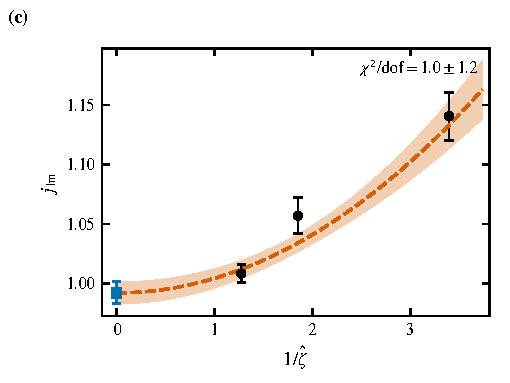
\includegraphics[width=\panelw]{figures/panels/extrap/par_ImA2B_j.pdf}\hfill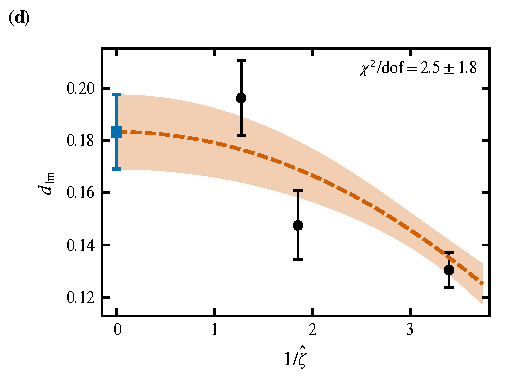
\includegraphics[width=\panelw]{figures/panels/extrap/par_ImA2B_d.pdf}\par
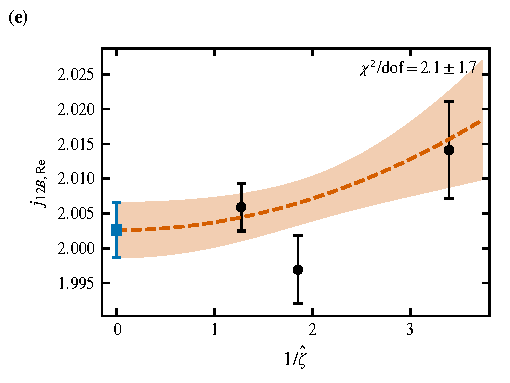
\includegraphics[width=\panelw]{figures/panels/extrap/par_ReA12B_j.pdf}\hfill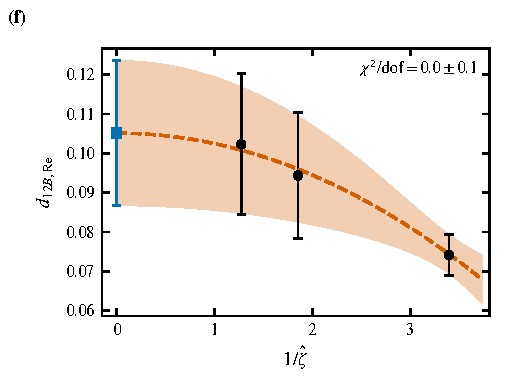
\includegraphics[width=\panelw]{figures/panels/extrap/par_ReA12B_d.pdf}
\caption{Extrapolation of the fit parameters $j$ and $d$ to $\hat\zeta\to\infty$ using $P_L=-2,-3,-4$ (black), with the ansatz $p_0+p_1/\hat\zeta^2$ (red dashed, band) and the extrapolated value (blue square). Panels (a, b) are for $\tAmp_{2B}^{\text{Re}}$, (c, d) for $\tAmp_{2B}^{\text{Im}}$ and (e, f) for $\tAmp_{12B}^{\text{Re}}$. Each panel gives the Jackknife $\chi^2/\text{dof}$.}
\label{fig:param_extrap_j}
\end{figure*}

\subsection{Factorization test on the lattice data}
\label{app:fact_data}

Figs.~\ref{fig:fact_data} and~\ref{fig:fact_data_P2} show the ratios $T$ and $B$ of Sec.~\ref{sec:factorization} for $P_L=-1$ and $-2$.

\begin{figure*}[!p]
\centering
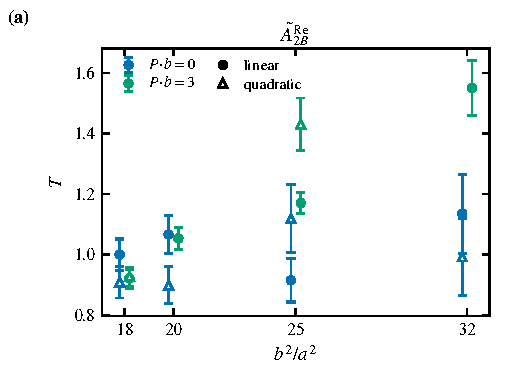
\includegraphics[width=\panelw]{figures/panels/fact/fd_PL1_ReA2B_T.pdf}\hfill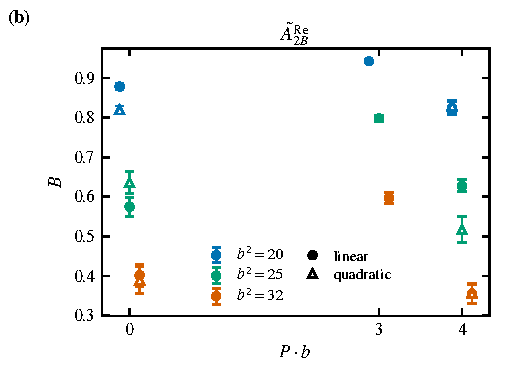
\includegraphics[width=\panelw]{figures/panels/fact/fd_PL1_ReA2B_B.pdf}\par
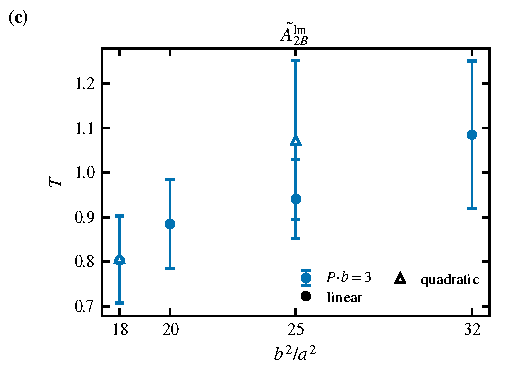
\includegraphics[width=\panelw]{figures/panels/fact/fd_PL1_ImA2B_T.pdf}\hfill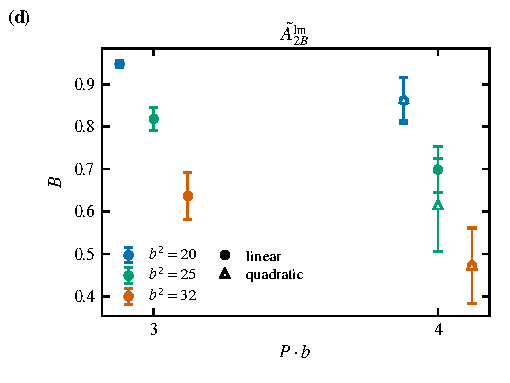
\includegraphics[width=\panelw]{figures/panels/fact/fd_PL1_ImA2B_B.pdf}\par
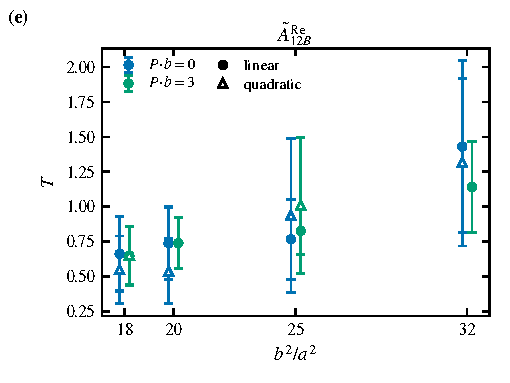
\includegraphics[width=\panelw]{figures/panels/fact/fd_PL1_ReA12B_T.pdf}\hfill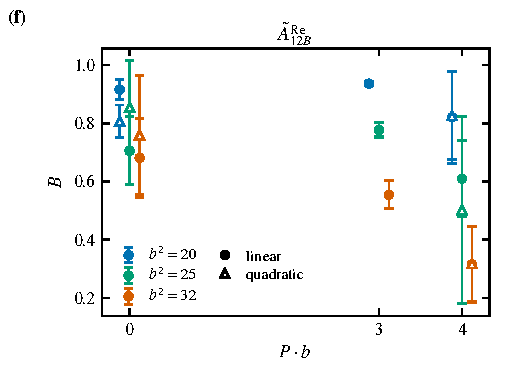
\includegraphics[width=\panelw]{figures/panels/fact/fd_PL1_ReA12B_B.pdf}
\caption{Factorization ratio test on the lattice data at $\eta|v|/a=8$, $P_L=-1$, for $\tAmp_{2B}^{\text{Re}}$, $\tAmp_{2B}^{\text{Im}}$ and $\tAmp_{12B}^{\text{Re}}$ (rows). Left: $T(P\cdot b,b^2)$ against $b^2$. Right: $B(P\cdot b,b^2)$ against $P\cdot b$. Under factorization every set of points is flat. Circles: linear interpolation in $b^2$. Triangles: quadratic interpolation on the $P\cdot b=0$ and $4$ rows. Errors are Jackknife errors and do not include the interpolation uncertainty.}
\label{fig:fact_data}
\end{figure*}

\begin{figure*}[!p]
\centering
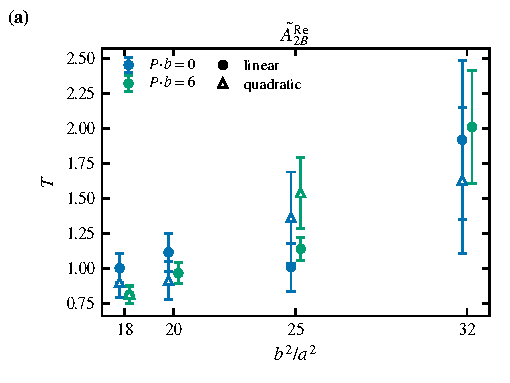
\includegraphics[width=\panelw]{figures/panels/fact/fd_PL2_ReA2B_T.pdf}\hfill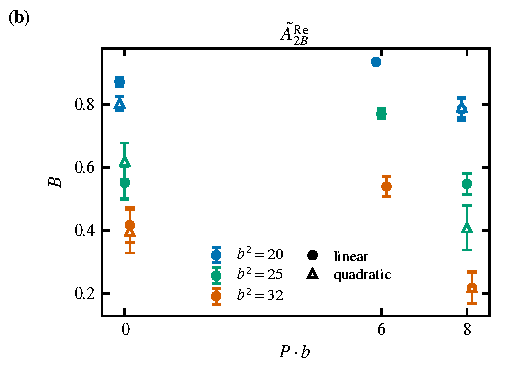
\includegraphics[width=\panelw]{figures/panels/fact/fd_PL2_ReA2B_B.pdf}\par
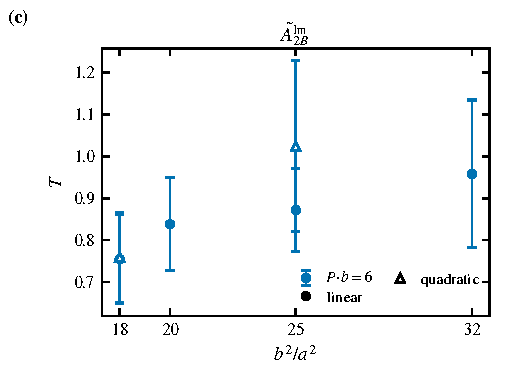
\includegraphics[width=\panelw]{figures/panels/fact/fd_PL2_ImA2B_T.pdf}\hfill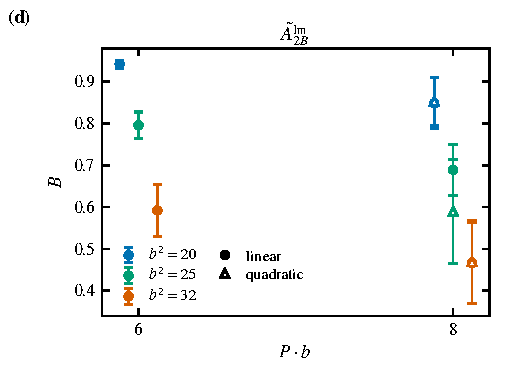
\includegraphics[width=\panelw]{figures/panels/fact/fd_PL2_ImA2B_B.pdf}\par
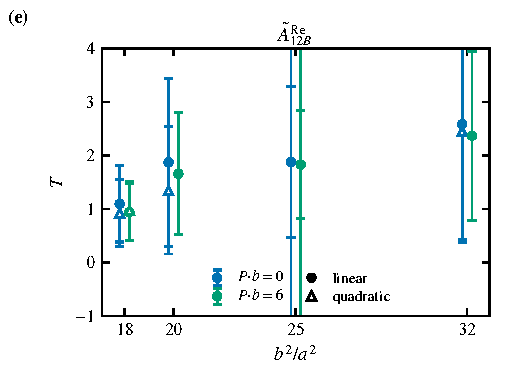
\includegraphics[width=\panelw]{figures/panels/fact/fd_PL2_ReA12B_T.pdf}\hfill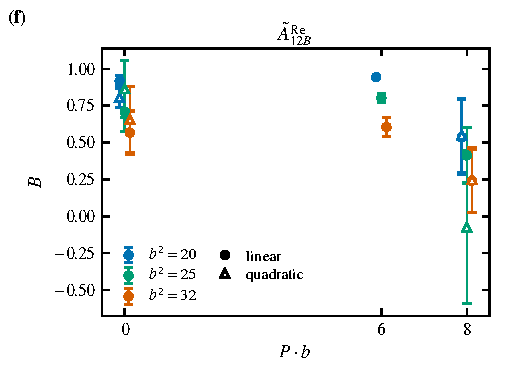
\includegraphics[width=\panelw]{figures/panels/fact/fd_PL2_ReA12B_B.pdf}
\caption{Same as Fig.~\ref{fig:fact_data}, but for $P_L=-2$ ($\hat\zeta=0.294367$). The lattice points are the same, with $P\cdot b=-P_Lb_L$ doubled. The reference row of $T$ is $P\cdot b=8$. In the $T$ panel for $\tAmp_{12B}^{\text{Re}}$ the quadratic ratio at $b^2=25$ has an error above $100$, because the reference row $P\cdot b=8$ crosses zero in some Jackknife samples; the vertical range is cut and this error bar extends beyond the frame.}
\label{fig:fact_data_P2}
\end{figure*}

\subsection{Amplitude data at $P_L=-3$ and $-4$}
\label{app:amps_blbt}
Extracted amplitudes as functions of $b_L/a$ and $b_T/a$ at $\vect{P}\cdot a\hat{L}/(2\pi)=\{-3,0,0\}$ and $\{-4,0,0\}$, in the format of Figs.~\ref{fig:BLBT_3D_P1}--\ref{fig:BLBT_eta8_P2}.

\begin{figure*}[!p]
\centering
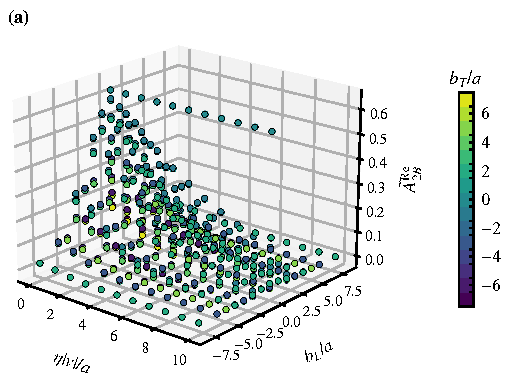
\includegraphics[width=\panelw]{figures/panels/amps/amp3d_ReA2B_PL3.pdf}\hfill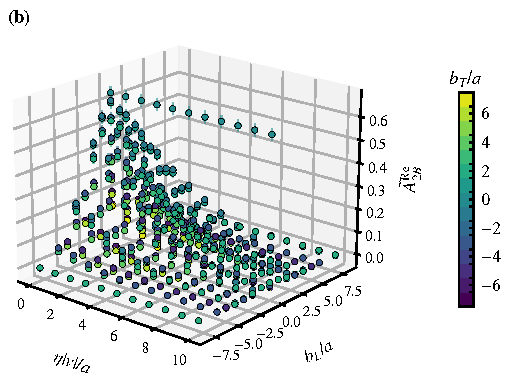
\includegraphics[width=\panelw]{figures/panels/amps/amp3d_ReA2B_PL4.pdf}\par
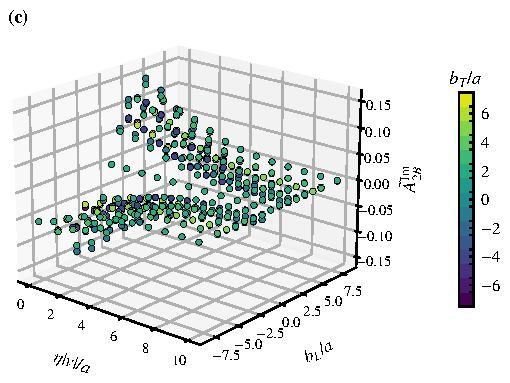
\includegraphics[width=\panelw]{figures/panels/amps/amp3d_ImA2B_PL3.pdf}\hfill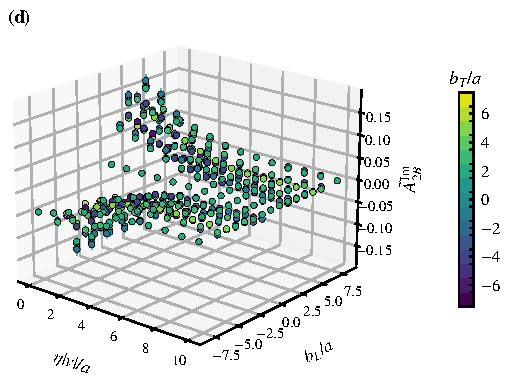
\includegraphics[width=\panelw]{figures/panels/amps/amp3d_ImA2B_PL4.pdf}\par
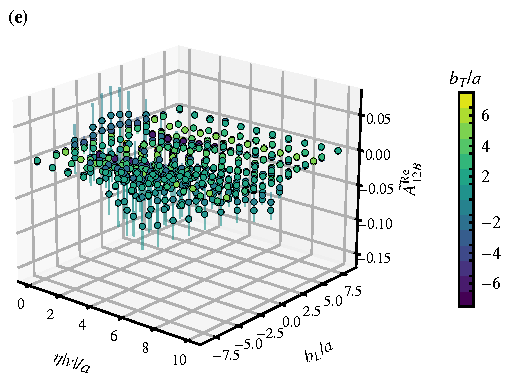
\includegraphics[width=\panelw]{figures/panels/amps/amp3d_ReA12B_PL3.pdf}\hfill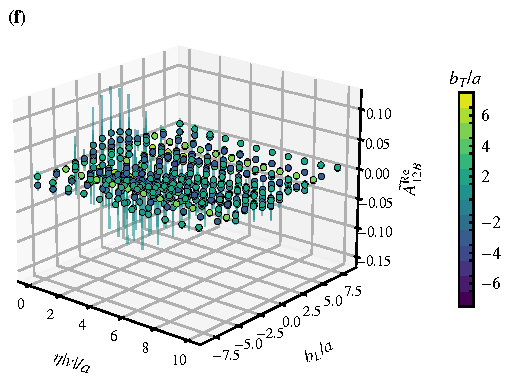
\includegraphics[width=\panelw]{figures/panels/amps/amp3d_ReA12B_PL4.pdf}
\caption{As Fig.~\ref{fig:BLBT_3D_P1} for $\vect{P}\cdot a\hat{L}/(2\pi)=\{-3,0,0\}$ ($\hat\zeta=0.539684$, left) and $\{-4,0,0\}$ ($\hat\zeta=0.785756$, right), rows: $\tAmp_{2B}^{\text{Re}}$, $\tAmp_{2B}^{\text{Im}}$, $\tAmp_{12B}^{\text{Re}}$.}
\label{fig:BLBT_3D_P3}
\end{figure*}

\begin{figure*}[!p]
\centering
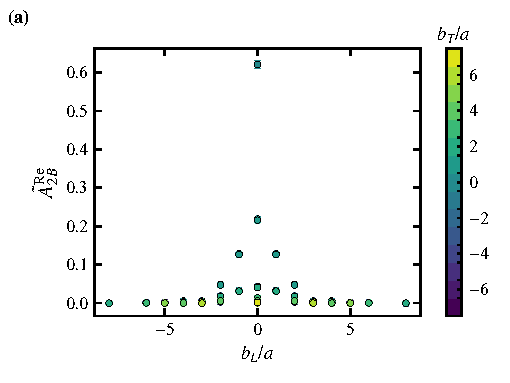
\includegraphics[width=\panelw]{figures/panels/amps/amp2d_eta8_ReA2B_PL3.pdf}\hfill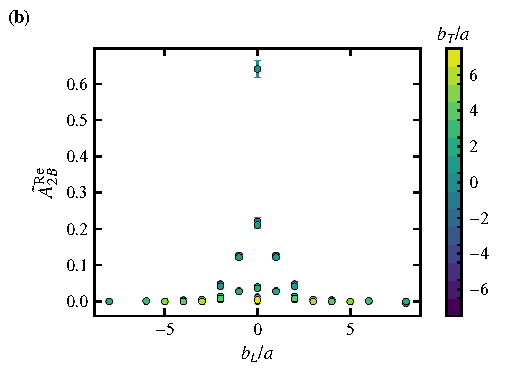
\includegraphics[width=\panelw]{figures/panels/amps/amp2d_eta8_ReA2B_PL4.pdf}\par
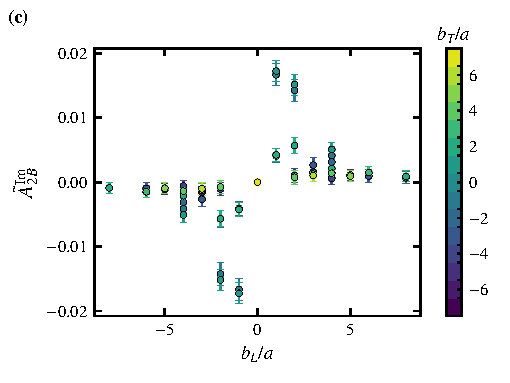
\includegraphics[width=\panelw]{figures/panels/amps/amp2d_eta8_ImA2B_PL3.pdf}\hfill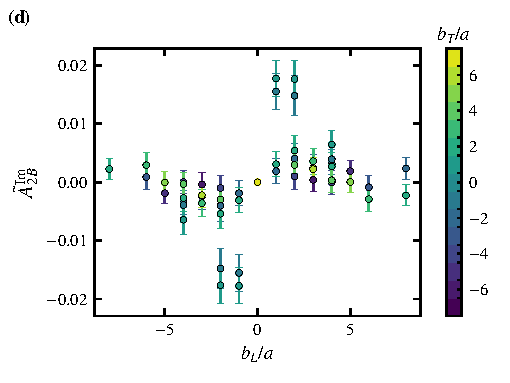
\includegraphics[width=\panelw]{figures/panels/amps/amp2d_eta8_ImA2B_PL4.pdf}\par
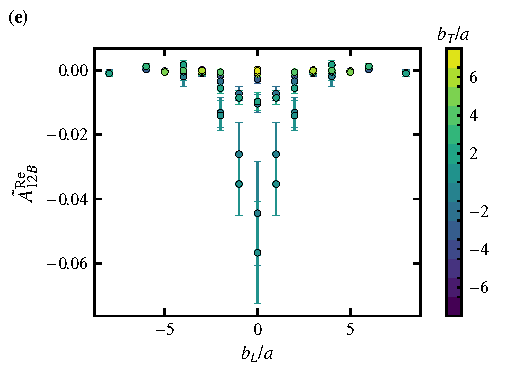
\includegraphics[width=\panelw]{figures/panels/amps/amp2d_eta8_ReA12B_PL3.pdf}\hfill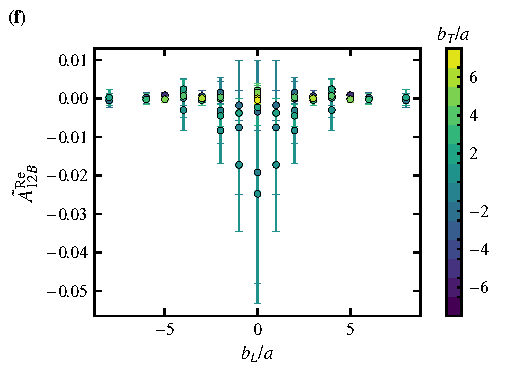
\includegraphics[width=\panelw]{figures/panels/amps/amp2d_eta8_ReA12B_PL4.pdf}
\caption{As Fig.~\ref{fig:BLBT_eta8_P1} for $\vect{P}\cdot a\hat{L}/(2\pi)=\{-3,0,0\}$ ($\hat\zeta=0.539684$, left) and $\{-4,0,0\}$ ($\hat\zeta=0.785756$, right), rows: $\tAmp_{2B}^{\text{Re}}$, $\tAmp_{2B}^{\text{Im}}$, $\tAmp_{12B}^{\text{Re}}$.}
\label{fig:BLBT_eta8_P3}
\end{figure*}

\begin{figure*}[!t]
\centering
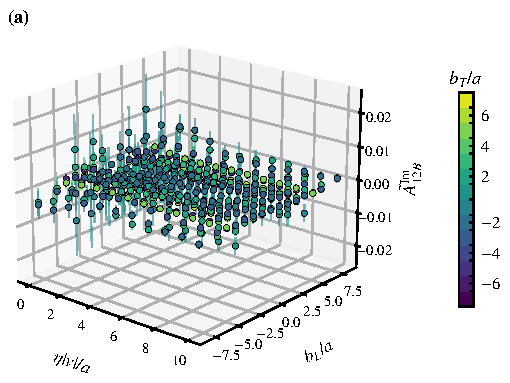
\includegraphics[width=\panelw]{figures/panels/amps/amp3d_ImA12B_PL3.pdf}\hfill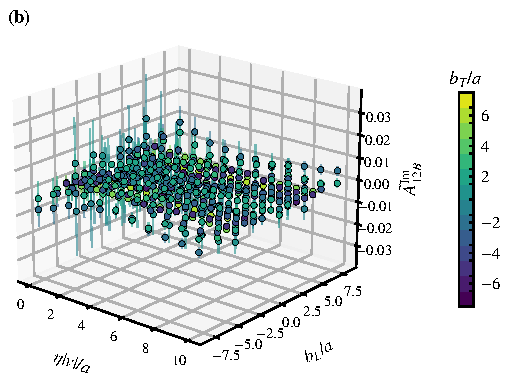
\includegraphics[width=\panelw]{figures/panels/amps/amp3d_ImA12B_PL4.pdf}\par
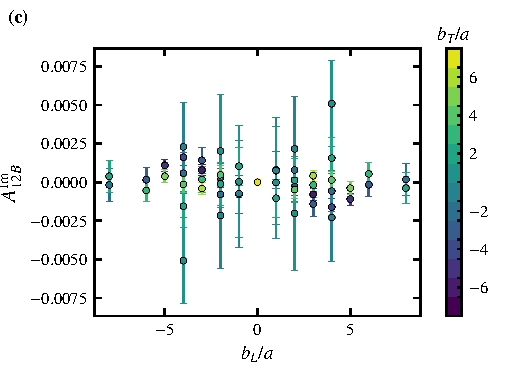
\includegraphics[width=\panelw]{figures/panels/amps/amp2d_eta8_ImA12B_PL3.pdf}\hfill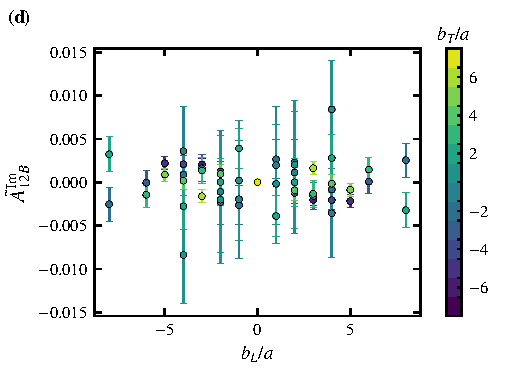
\includegraphics[width=\panelw]{figures/panels/amps/amp2d_eta8_ImA12B_PL4.pdf}
\caption{$\tAmp_{12B}^{\text{Im}}$ for $\vect{P}\cdot a\hat{L}/(2\pi)=\{-3,0,0\}$ ($\hat\zeta=0.539684$, left) and $\{-4,0,0\}$ ($\hat\zeta=0.785756$, right): as functions of $\eta|\vect v|/a$ and $b_L/a$ (top) and of $b_L/a$ at $\eta|\vect v|/a=8$ (bottom).}
\label{fig:BLBT_ImA12B_P34}
\end{figure*}
